\documentclass[11pt]{article}
\usepackage{amsmath,amssymb,amsthm}
\usepackage{fullpage}
\usepackage{graphicx}
\usepackage{algorithm}
\usepackage[noend]{algpseudocode}
\usepackage{tikz}
\usepackage[hidelinks]{hyperref}
\usepackage{caption}
\usepackage{subcaption}

\newtheorem{theorem}{Theorem}

\title{Dynamic Programming for Polynomial-Time Subset Selection in 1-D and 2-D Non Dominated Sets via Riesz 
s-Energy Minimization}
\author{Michael Emmerich\\Faculty of IT, University of Jyväskylä, Finland}
\date{\today}

\begin{document}

\maketitle

\begin{abstract}
  We present a dynamic programming algorithm for selecting a representative subset of points from a given dataset such that the Riesz \(s\)-energy is minimized. In the one-dimensional case, the natural ordering of the data allows for an efficient recursion. This approach is then extended to two-dimensional Pareto fronts arising in biobjective optimization problems. The proposed methods guarantee an optimal solution under the assumption of sorted (or non-dominated) input, and the overall time complexity is shown to be \(O(n^2 k)\) when suitable precomputation is applied.
  
  \bigskip
  \noindent\textbf{Keywords:} Dynamic Programming, Subset Selection, Riesz \(s\)-Energy, Pareto Front, Biobjective Optimization.
\end{abstract}

\section{Introduction}

In many optimization problems it is desirable to select a representative subset of points such that the points are as evenly spread as possible. A common measure to quantify this evenness is the \emph{Riesz \(s\)-energy}. For a set \(S\) of \(k\) points, the Riesz \(s\)-energy is defined as
\[
E(S)=\sum_{1\le p<q\le k}\frac{1}{d(P_p,P_q)^s},
\]
where \(d(P_p,P_q)\) denotes the distance between the points \(P_p\) and \(P_q\) and \(s>0\) is a parameter. In this paper we describe a dynamic programming (DP) approach to select a subset that minimizes the Riesz \(s\)-energy. We begin with the one-dimensional (1D) case (points on the real line) and then extend the technique to two-dimensional (2D) Pareto fronts in the context of biobjective optimization.

It is worth noting that while the general problem is NP-hard \cite{Pereverdieva2024}, in the 1D case (or for suitably ordered 2D Pareto fronts) the structure of the data permits an efficient DP formulation.

\section{Dynamic Programming for Subset Selection in 1D}

\subsection{Problem Statement}

Let 
\[
x_1 < x_2 < \cdots < x_n
\]
be a sorted set of points in \(\mathbb{R}\). For a given integer \(k\) (\(1 \le k < n\)) and a parameter \(s>0\), our goal is to choose a subset 
\[
S = \{ x_{i_1}, x_{i_2}, \dots, x_{i_k} \}, \quad \text{with } i_1 < i_2 < \cdots < i_k,
\]
that minimizes
\[
E(S) = \sum_{1 \le p < q \le k} \frac{1}{\left(x_{i_q} - x_{i_p}\right)^s}.
\]
Since the energy increases sharply when points are close (due to the term \(1/(x_{i_q}-x_{i_p})^s\)), the objective is to select \(k\) points that are as spread out as possible.

\subsection{Dynamic Programming Algorithm}

We define the DP state as
\[
DP(i,r)=\text{minimum energy achievable by selecting \(r\) points from } \{x_1, \dots, x_i\} \text{ with } x_i \text{ as the last point.}
\]

\paragraph{Base Case:} For \(r=1\), there are no pairs of points, hence 
\[
DP(i,1)=0 \quad \text{for } i=1,\dots,n.
\]

\paragraph{Recurrence:} For \(r\ge2\) and \(i\ge r\), assume an optimal \((r-1)\)-subset ending at \(x_p\) (with \(p < i\)) is known. When adding \(x_i\) as the \(r\)th point, the additional cost is
\[
\Delta(p,i)=\sum_{x \in S(p,r-1)} \frac{1}{(x_i - x)^s},
\]
where \(S(p,r-1)\) denotes the optimal subset corresponding to \(DP(p, r-1)\). Hence, the recurrence is
\[
DP(i,r)=\min_{1 \le p < i} \left\{ DP(p,r-1) + \Delta(p,i) \right\}.
\]

\subsubsection*{Pseudocode}

\begin{algorithm}[H]
\caption{DP Subset Selection for Minimizing Riesz \(s\)-Energy in 1D}\label{alg:dp1d}
\begin{algorithmic}[1]
\Require Sorted points \(x_1,\dots,x_n\), integer \(k\), parameter \(s>0\).
\For{\(i=1\) to \(n\)}
    \State \(DP(i,1) \gets 0\)
    \State \(S(i,1) \gets \{ x_i \}\) \Comment{Record the subset for reconstruction.}
\EndFor
\For{\(r = 2\) to \(k\)}
    \For{\(i = r\) to \(n\)}
        \State \(DP(i,r) \gets +\infty\)
        \For{\(p = r-1\) to \(i-1\)}
            \State Compute \(\Delta(p,i) \gets \sum_{x\in S(p,r-1)} \frac{1}{(x_i - x)^s}\)
            \If{\(DP(p,r-1)+\Delta(p,i) < DP(i,r)\)}
                \State \(DP(i,r) \gets DP(p,r-1)+\Delta(p,i)\)
                \State \(S(i,r) \gets S(p,r-1) \cup \{ x_i \}\)
            \EndIf
        \EndFor
    \EndFor
\EndFor
\State \Return \(\min_{i=k,\dots,n} DP(i,k)\) and the corresponding subset.
\end{algorithmic}
\end{algorithm}

\subsection{Proof of Correctness}

We prove by induction on \(r\) that for every state \(DP(i,r)\) the algorithm computes the minimum energy achievable by selecting \(r\) points from \(\{x_1,\dots,x_i\}\) with \(x_i\) as the last point.

\paragraph{Base Case (\(r=1\)):}  
For \(r=1\) the energy is zero (no pairs exist), and the initialization \(DP(i,1)=0\) is correct.

\paragraph{Inductive Step:}  
Assume the DP values are correct for \(r-1\). For an optimal subset 
\[
S = \{x_{i_1}, x_{i_2}, \dots, x_{i_{r-1}}, x_i\},
\]
with \(x_{i_{r-1}}=x_p\), the total energy is
\[
DP(p, r-1) + \Delta(p,i),
\]
where
\[
\Delta(p,i)=\sum_{j=1}^{r-1}\frac{1}{\left(x_i - x_{i_j}\right)^s}.
\]
Minimizing over all valid \(p\) yields the recurrence. Hence, by induction, the algorithm finds the optimal solution.

\subsection{Time Complexity}

The DP table is of size \(O(nk)\) and for each state \(DP(i,r)\) the algorithm examines up to \(O(n)\) previous states. With appropriate precomputation (or memoization) of the \(\Delta(p,i)\) values, the overall time complexity is \(O(n^2 k)\).

\subsection{Examples}

\subsubsection*{Example 1: \(x=[0,\,1,\,3,\,6]\), \(k=3\), \(s=1\)}

\begin{itemize}
    \item \(\{0,1,3\}\): 
    \[
    E= \frac{1}{1-0}+\frac{1}{3-0}+\frac{1}{3-1}= 1 + \frac{1}{3} + \frac{1}{2} \approx 1.8333.
    \]
    \item \(\{0,1,6\}\): 
    \[
    E= 1 + \frac{1}{6-0} + \frac{1}{6-1} \approx 1.3667.
    \]
    \item \(\{0,3,6\}\): 
    \[
    E= \frac{1}{3-0} + \frac{1}{6-0} + \frac{1}{6-3} \approx 0.8333.
    \]
    \item \(\{1,3,6\}\):  
    \[
    E \approx 1.0333.
    \]
\end{itemize}

Thus, the optimal subset is \(\{0,3,6\}\) with an energy of approximately \(0.8333\).

\section{Dynamic Programming for Subset Selection on 2D Pareto Fronts}

\subsection{Introduction}

In many biobjective optimization problems, the goal is to approximate the Pareto front --- a set of non-dominated solutions --- with a representative subset. Although the Pareto front is two-dimensional, when the points are sorted by one coordinate (typically \(f_1\)) the other coordinate (\(f_2\)) follows a monotonic order. This observation allows us to extend the 1D DP scheme to the 2D case.

\subsection{Problem Statement}

Let
\[
P_1, P_2, \dots, P_n \in \mathbb{R}^2
\]
be a set of non-dominated points, sorted such that 
\[
f_1(P_1) \le f_1(P_2) \le \cdots \le f_1(P_n)
\]
and, because of non-domination, 
\[
f_2(P_1) \ge f_2(P_2) \ge \cdots \ge f_2(P_n).
\]
For a given integer \(k\) (\(1 \le k < n\)) and a parameter \(s>0\), we wish to select a subset
\[
S=\{P_{i_1},P_{i_2},\dots,P_{i_k}\}, \quad i_1 < i_2 < \cdots < i_k,
\]
that minimizes
\[
E(S)=\sum_{1\le p<q\le k}\frac{1}{d(P_{i_p},P_{i_q})^s},
\]
where \(d(P,Q)\) denotes the Euclidean distance between points \(P\) and \(Q\).

\subsection{Dynamic Programming Algorithm}

Similarly, we define the DP state by
\[
DP(i,r)=\text{minimum energy attainable by selecting \(r\) points from } \{P_1,\dots,P_i\} \text{ with } P_i \text{ as the last point.}
\]
We also record the corresponding subset \(S(i,r)\).

\paragraph{Base Case:} For \(r=1\),
\[
DP(i,1)=0 \quad \text{for } i=1,\dots,n,
\]
with \(S(i,1)=\{P_i\}\).

\paragraph{Recurrence:} For \(r\ge2\) and \(i\ge r\), assume an optimal \((r-1)\)-subset ending at \(P_p\) (with \(p < i\)) is computed. When adding \(P_i\), the incremental cost is given by
\[
\Delta(p,i)=\sum_{P\in S(p,r-1)} \frac{1}{d(P,P_i)^s}.
\]
Thus, the recurrence becomes
\[
DP(i,r)=\min_{p=r-1,\ldots,i-1}\{DP(p,r-1)+\Delta(p,i)\},
\]
with
\[
S(i,r)=S(p,r-1)\cup\{P_i\}.
\]

\subsubsection*{Pseudocode}

\begin{algorithm}[H]
\caption{DP Subset Selection for Minimizing Riesz \(s\)-Energy on a 2D Pareto Front}\label{alg:dp2d}
\begin{algorithmic}[1]
\Require Non-dominated points \(P_1,\dots,P_n \in \mathbb{R}^2\) sorted such that 
\[
f_1(P_1) \le \cdots \le f_1(P_n) \quad\text{and}\quad f_2(P_1) \ge \cdots \ge f_2(P_n),
\]
integer \(k\), parameter \(s>0\).
\For{\(i=1\) to \(n\)}
    \State \(DP(i,1) \gets 0\)
    \State \(S(i,1) \gets \{P_i\}\)
\EndFor
\For{\(r = 2\) to \(k\)}
    \For{\(i = r\) to \(n\)}
        \State \(DP(i,r) \gets +\infty\)
        \For{\(p = r-1\) to \(i-1\)}
            \State Compute \(\Delta(p,i) \gets \displaystyle \sum_{P\in S(p,r-1)} \frac{1}{d(P,P_i)^s}\)
            \If{\(DP(p,r-1)+\Delta(p,i) < DP(i,r)\)}
                \State \(DP(i,r) \gets DP(p,r-1)+\Delta(p,i)\)
                \State \(S(i,r) \gets S(p,r-1)\cup\{P_i\}\)
            \EndIf
        \EndFor
    \EndFor
\EndFor
\State \Return \(\min_{i=k,\dots,n}\{DP(i,k)\}\) and the corresponding subset.
\end{algorithmic}
\end{algorithm}

\subsection{Theorem and Proof of Correctness}

\begin{theorem}
Let \(P_1,\dots,P_n \in \mathbb{R}^2\) be non-dominated points sorted by increasing \(f_1\) (and, consequently, decreasing \(f_2\)). Then Algorithm~\ref{alg:dp2d} computes an optimal subset \(S\) of size \(k\) that minimizes
\[
E(S)=\sum_{1\le p<q\le k}\frac{1}{d(P_{i_p},P_{i_q})^s}.
\]
\end{theorem}

\begin{proof}
Because the points are sorted by \(f_1\) and are non-dominated (ensuring \(f_2\) is in descending order), for any \(i<j\) we have
\[
f_1(P_i) \le f_1(P_j) \quad \text{and} \quad f_2(P_i) \ge f_2(P_j).
\]
This ordering implies a lower bound \(d(P_i,P_j) \ge f_1(P_j)-f_1(P_i)\) and ensures that the additional cost incurred by adding a new point is monotonic with respect to the ordering. Consequently, any optimal \(r\)-subset ending at \(P_i\) can be constructed from an optimal \((r-1)\)-subset ending at some \(P_p\) (with \(p < i\)) plus the cost \(\Delta(p,i)\). By induction, the recurrence 
\[
DP(i,r)=\min_{p< i}\{DP(p,r-1)+\Delta(p,i)\}
\]
yields the overall optimal energy.
\end{proof}

\subsection{Example: Biobjective Optimization}

Consider the following set of non-dominated points:
\[
P_1=(1,15),\quad P_2=(5,10),\quad P_3=(8,4),\quad P_4=(13,3),\quad P_5=(15,2),\quad P_6=(17,1).
\]
They are sorted by the first coordinate. Suppose we wish to select \(k=3\) points. One candidate selected by the DP approach is 
\[
S=\{P_1,P_3,P_6\}=\{(1,15),(8,4),(17,1)\}.
\]
With approximate pairwise distances:
\[
d(P_1,P_3)\approx 13.04,\quad d(P_1,P_6)\approx 21.26,\quad d(P_3,P_6)\approx 9.49,
\]
the energy (with \(s=1\)) is approximately
\[
E(S)\approx \frac{1}{13.04}+\frac{1}{21.26}+\frac{1}{9.49}\approx 0.229.
\]

%\subsection{Illustrations}

\begin{figure}[htb]
  \centering
  \begin{minipage}{0.5\textwidth}
    \centering
    % TikZ Illustration for Example 1
    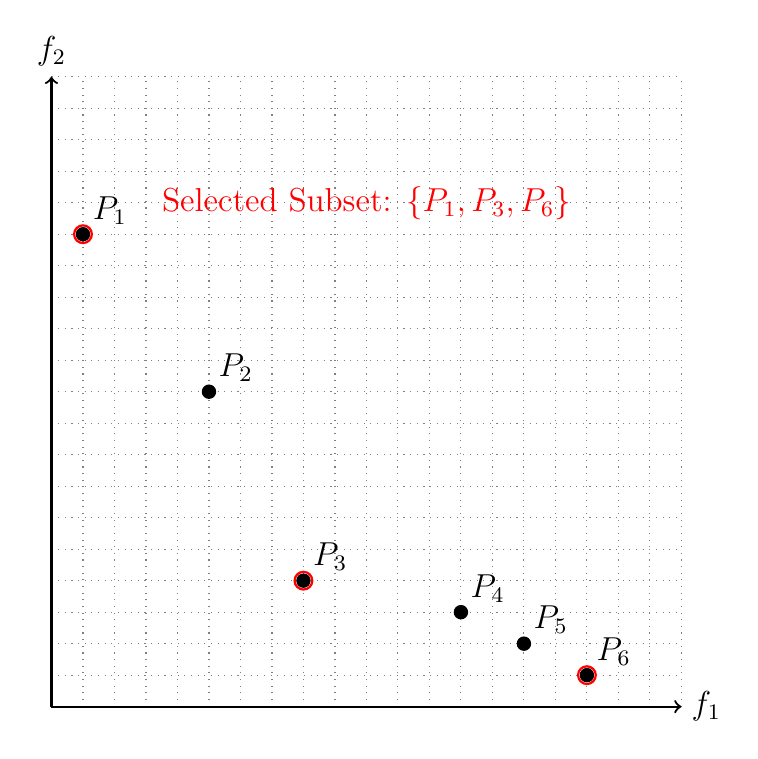
\begin{tikzpicture}[scale=0.4, every node/.style={font=\large}]
      % Dotted grid (20x20)
      \draw[dotted, step=1, gray] (0,0) grid (20,20);
      \draw[->, thick] (0,0) -- (20,0) node[right] {\(f_1\)};
      \draw[->, thick] (0,0) -- (0,20) node[above] {\(f_2\)};
      
      % Plot Pareto points with larger points
      \foreach \x/\y/\name in {1/15/\(P_1\), 5/10/\(P_2\), 8/4/\(P_3\), 13/3/\(P_4\), 15/2/\(P_5\), 17/1/\(P_6\)}
      {
        \draw[black, fill=black] (\x,\y) circle (6pt);
        \node[above right] at (\x,\y) {\name};
      }
      
      % Highlight the selected subset
      \foreach \x/\y in {1/15, 8/4, 17/1}
      {
        \draw[red, thick] (\x,\y) circle (8pt);
      }
      
      % Optional label for the selected subset
      \node[red] at (10,16) {Selected Subset: \(\{P_1,P_3,P_6\}\)};
    \end{tikzpicture}
    \caption*{Example 1: Pareto front with selected subset \(\{P_1,P_3,P_6\}\).}
  \end{minipage}%
  \hfill
  \begin{minipage}{0.5\textwidth}
    \centering
    % TikZ Illustration for Additional Example
    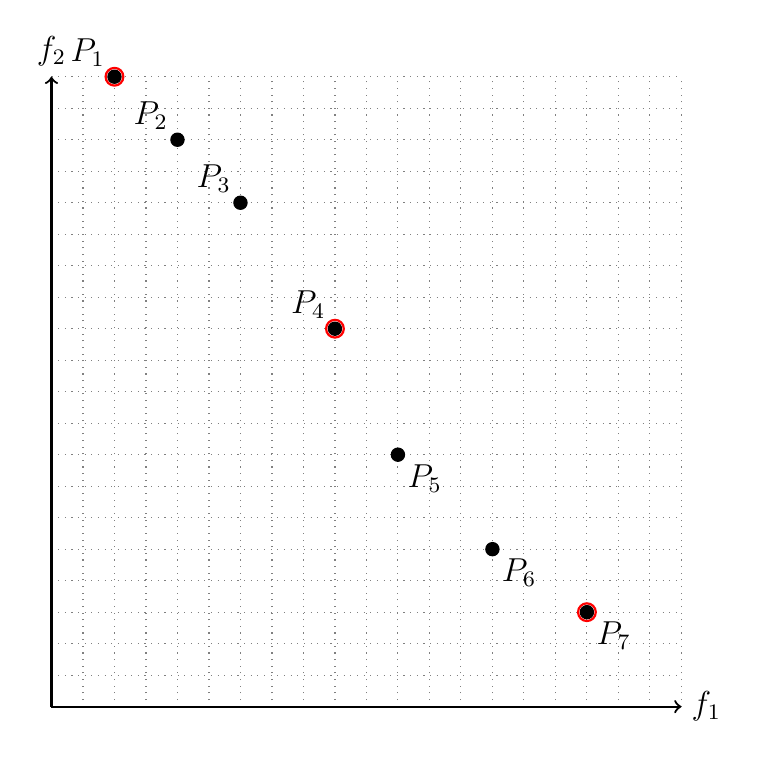
\begin{tikzpicture}[scale=0.4, every node/.style={font=\large}]
      % Dotted grid (20x20)
      \draw[dotted, step=1, gray] (0,0) grid (20,20);
      \draw[->, thick] (0,0) -- (20,0) node[right] {\(f_1\)};
      \draw[->, thick] (0,0) -- (0,20) node[above] {\(f_2\)};
      
      % Plot all points with larger points
      \draw[black, fill=black] (2,20) circle (6pt) node[above left] {\(P_1\)};
      \draw[black, fill=black] (4,18) circle (6pt) node[above left] {\(P_2\)};
      \draw[black, fill=black] (6,16) circle (6pt) node[above left] {\(P_3\)};
      \draw[black, fill=black] (9,12) circle (6pt) node[above left] {\(P_4\)};
      \draw[black, fill=black] (11,8) circle (6pt) node[below right] {\(P_5\)};
      \draw[black, fill=black] (14,5) circle (6pt) node[below right] {\(P_6\)};
      \draw[black, fill=black] (17,3) circle (6pt) node[below right] {\(P_7\)};
      
      % Highlight selected points
      \draw[red, thick] (2,20) circle (8pt);
      \draw[red, thick] (9,12) circle (8pt);
      \draw[red, thick] (17,3) circle (8pt);
    \end{tikzpicture}
    \caption*{Additional Example: Pareto front with selected subset \(\{P_1,P_4,P_7\}\).}
  \end{minipage}
  \caption{DP-selected representative subsets on two Pareto front examples.}
\end{figure}

\section{Conclusion}

We have presented a dynamic programming algorithm for subset selection that minimizes the Riesz \(s\)-energy in both one-dimensional and two-dimensional settings. In the 1D case the inherent ordering of the data leads to a straightforward DP formulation, while for 2D Pareto fronts the proper sorting (by increasing \(f_1\) and decreasing \(f_2\)) permits a similar approach. With a time complexity of \(O(n^2 k)\) (assuming constant-time updates via precomputation), the method offers an effective strategy for selecting representative subsets in various applications.

\bibliographystyle{plain}
\begin{thebibliography}{1}
\bibitem{Pereverdieva2024} Pereverdieva, K., Deutz, A., Ezendam, T., Bäck, T., Hofmeyer, H., \& Emmerich, M. (2024). \emph{Comparative Analysis of Indicators for Multiobjective Diversity Optimization}. arXiv preprint \href{https://arxiv.org/abs/2410.18900}{arXiv:2410.18900}.
\end{thebibliography}

\end{document}
